\setcounter{chapter}{7}
\chapter{Podsumowanie i wnioski końcowe}
\label{chap:podsumowanie-wnioski-koncowe}

\providecommand{\ChapterEightFigure}[3]{%
\begin{figure}[htbp]
\centering
\IfFileExists{#1}{%
    \includegraphics[width=0.92\textwidth]{#1}%
}{%
    \fbox{%
        \begin{minipage}[c][0.25\textheight][c]{0.86\textwidth}
        \centering
        \small Brak pliku graficznego w repozytorium:\\[4pt]
        {\scriptsize\texttt{\detokenize{#1}}}
        \end{minipage}%
    }%
}%
\caption{#2}
\label{#3}
\end{figure}%
}

Ostatni rozdział pracy stanowi syntezę przeprowadzonych badań, ocenę stopnia realizacji założonych celów oraz wskazanie obszarów wymagających dalszej eksploracji w przyszłości.

Głównym celem niniejszej pracy było zbadanie możliwości wykorzystania technik uczenia maszynowego do przewidywania adopcyjności i czasu pobytu zwierząt, czyli psów i kotów, w schronisku typu \emph{No-Kill} na podstawie danych dostępnych wyłącznie w momencie ich przyjęcia. Wyniki eksperymentów, oparte na analizie ponad 160 tysięcy epizodów z Austin Animal Center, wskazują na wysoką skuteczność analityczną zastosowanych algorytmów z rodziny drzew decyzyjnych, w szczególności modeli \emph{Gradient Boosting}. Zbudowane modele pozwalają identyfikować wzorce związane z późniejszym losem zwierzęcia.

\section{Odpowiedzi na pytania badawcze i weryfikacja hipotez}
\label{sec:odpowiedzi-na-pytania-badawcze-hipotezy}

W toku prowadzonych eksperymentów zweryfikowano trzy kluczowe pytania badawcze (RQ), które ukierunkowały niniejszą pracę:

\begin{description}
    \item[RQ1: Jakie cechy zwierzęcia są najważniejszymi predyktorami adopcyjności?] \hfill \\
    Analiza ważności cech, wsparta wyjaśnieniami SHAP, wskazała spójnie, że najważniejszymi predyktorami pozytywnej adopcyjności i krótkiego czasu pobytu są imię zwierzęcia (zmienna \texttt{has\_name}) oraz jego wiek. Młodsze zwierzęta posiadające nadane imię w momencie przyjęcia mają znacznie większe szanse na pozytywne zakończenie epizodu schroniskowego. Tradycyjne cechy fizyczne, takie jak kategoria rasy czy umaszczenie (kolor), odgrywają w ogólnym rozrachunku rolę drugorzędną.
    
    \item[RQ2: Czy zaawansowane modele (Gradient Boosting) przewyższają linie bazowe?] \hfill \\
    Eksperymenty pokazały jednoznaczną przewagę zaawansowanych algorytmów drzewiastych nad metodami bazowymi. W~klasyfikacji adopcji najlepszy okazał się model \emph{HistGradientBoosting}, uzyskując PR-AUC równe 0,884 oraz ROC-AUC na poziomie 0,840, wyraźnie przewyższając regresję logistyczną~\cite{Grinsztajn2022}. W~zadaniu regresyjnym najniższy błąd osiągnął \emph{CatBoost} (MAE = 18,55~dnia). Potwierdza to, że drzewa decyzyjne z boostingiem gradientowym skutecznie wychwytują nieliniowe zależności pomiędzy atrybutami schroniskowymi.
    
    \item[RQ3: Jak zjawiska makrostrukturalne oraz różnice gatunkowe wpływają na wzorce?] \hfill \\
    Zidentyfikowano wyraźne różnice w zdolności predykcyjnej dla poszczególnych gatunków: skuteczność modeli była wyższa dla kotów (PR-AUC na poziomie 0,899) niż dla psów (PR-AUC 0,857), co sugeruje, że psy bywają oceniane przez pryzmat bardziej złożonych preferencji i cech niewidocznych w systemie (np. behawioralnych). Dodatkowo wykazano, że okres pandemii COVID-19 w istotny sposób zmodyfikował przepływ zwierząt w schronisku, wydłużając czas ich pobytu i modyfikując dynamikę rotacji jako bardzo silna zmienna zakłócająca (confounder).
\end{description}

\begin{figure}[htbp]
\centering
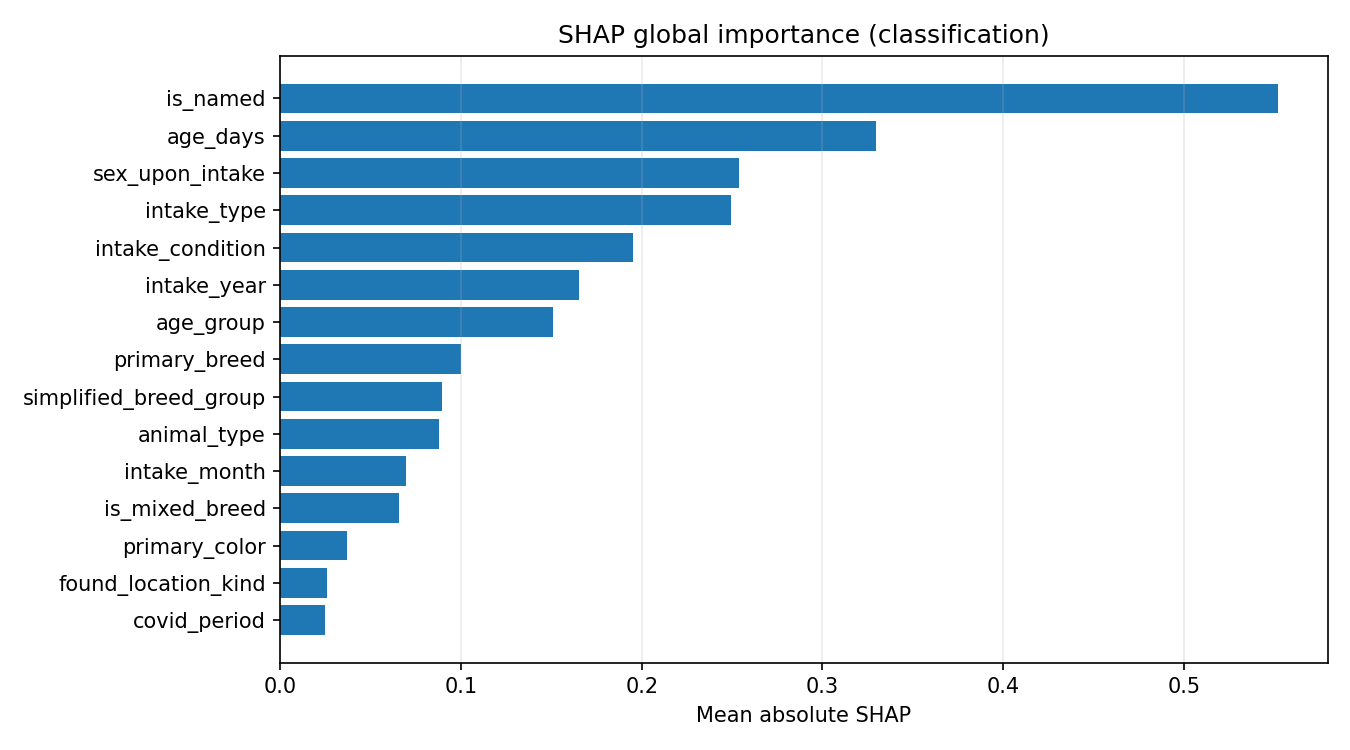
\includegraphics[width=0.88\textwidth]{../reports/figures/shap_summary_classification.png}
\caption{Globalny wykres wartości SHAP dla modelu klasyfikacyjnego, potwierdzający dominującą rolę zmiennej \texttt{has\_name}, wieku oraz typu przyjęcia w~kształtowaniu prawdopodobieństwa adopcji.}
\label{fig:shap-ch8-rq1}
\end{figure}

\section{Ograniczenia badawcze i metodologiczne}
\label{sec:ograniczenia-badawcze-metodologiczne}

Ocena modeli predykcyjnych wymaga wskazania ich ograniczeń.

\begin{enumerate}
    \item \textbf{Cenzorowanie prawostronne (\emph{Right-Censoring}).} Do trenowania klasycznych algorytmów predykcyjnych, w szczególności regresji długości pobytu, konieczne było pominięcie epizodów, które nie posiadały wpisanego wyniku zakończenia w momencie zrzutu bazy danych. Zjawisko to jest ograniczeniem wynikającym z odstąpienia od technik analizy przeżycia (\emph{Survival Analysis}).
    \item \textbf{Specyfika schronisk typu \emph{No-Kill} i generalizowalność (\emph{Single-Shelter Generalizability}).} Zidentyfikowane wzorce odnoszą się do placówki działającej w środowisku o wysokiej świadomości społecznej (Austin, Teksas). Przeniesienie modelu do schroniska o innej polityce demograficznej i mniejszych zasobach finansowych mogłoby prowadzić do spadku skuteczności z powodu odmiennych wzorców.
    \item \textbf{Brak zmiennych behawioralnych.} Zgodnie z założeniem predykcji tuż po przyjęciu (\emph{intake-only}), w wektorze wejściowym nie zawarto oceny behawioralnej zwierzęcia, co w pewnych przypadkach ogranicza sprawność modeli.
    \item \textbf{Implikacje etyczne (\emph{Ethical Implications}).} Używanie modeli ML do wskazywania profili wysokiego ryzyka niesie potencjalne niebezpieczeństwo stygmatyzacji. Błędnie przewidziane wysokie ryzyko długiego pobytu mogłoby zniechęcić personel do inwestowania czasu w dane zwierzę, tworząc samospełniającą się przepowiednię.
    \item \textbf{Uprzedzenia w etykietowaniu ras (\emph{Breed Labeling Bias}).} Identyfikacja ras w schroniskach odbywa się często w sposób subiektywny na podstawie wyglądu (\emph{visual breed identification}). Może to prowadzić do zaburzenia percepcji ras wprowadzanych do wektorów wejściowych modelu.
    \item \textbf{Luki w kalibracji w zależności od grupy (\emph{Calibration Gaps by Cohort}).} Choć ogólna skuteczność modelu jest wysoka, występują różnice w kalibracji dla mniejszych, specyficznych grup (np. wybrane grupy psów), co po wdrożeniu operacyjnym może zmniejszyć pewność modeli w pojedynczych kohortach.
    \item \textbf{Pandemia jako czynnik zakłócający (\emph{COVID Confounders}).} Pandemia COVID-19 drastycznie zmieniła zachowania adoptujących oraz politykę przyjęć. Brak uwzględnienia odpowiednio skompensowanych wskaźników tej makro-zmiennej może powodować problemy w analizie po pandemii.
\end{enumerate}

\section{Kierunki dalszych badań i rekomendacje praktyczne}
\label{sec:kierunki-dalszych-badan-future-work}

Rezultaty uzyskane w niniejszej pracy wskazują na możliwość dalszego rozwijania projektu w kierunku naukowym i wdrożeniowym:

\begin{itemize}
    \item \textbf{Uczenie transferowe (\emph{Transfer Learning}).} Próba przeniesienia modeli wytrenowanych na bazie z Austin do innej, mniejszej placówki pozwoliłaby na ocenę podatności zbudowanych architektur na wiedzę dziedzinową schronisk na szerszą skalę.
    \item \textbf{Integracja z danymi w czasie rzeczywistym (\emph{Real-Time Data Integration}).} Stworzenie asynchronicznego API połączonego z klasycznym oprogramowaniem ewidencyjnym schroniska, by asystent predykcyjny klasyfikował przypadki już minutę po dokonaniu rejestracji.
    \item \textbf{Wykorzystanie widzenia komputerowego (\emph{Computer Vision}).} Ocena potencjału zdjęć zwierząt przy pomocy sieci wizyjnych do przechwytywania walorów estetycznych z fotografii, które silnie wpływają na wizerunek rynkowy i skłonności adoptujących.
    \item \textbf{Integracja z mediami społecznościowymi (\emph{Social Media Integration}).} Podłączenie oprogramowania flagującego do automatycznych akcji promocyjnych online w celu aktywnego dystrybuowania materiałów o trudnych zwierzętach na zewnętrznych platformach.
    \item \textbf{Ewaluacja wariantu wdrożeniowego (Testy A/B).} Rzeczywiste eksperymenty losowe (A/B testing) z modelem w schronisku na oddzielonej grupie kontrolnej mogłyby definitywnie potwierdzić zdolność systemu do przyspieszenia procesu operacyjnego, izolując narzędzie od efektów psychologicznych.
\end{itemize}

\subsection{Rekomendacje dla personelu schronisk}

Obok perspektyw teoretycznych sformułowano wytyczne, z których personel placówek zyska korzyści poprzez korektę bieżących działań na poziomie zarządczym:
\begin{itemize}
    \item \textbf{Flagowanie przypadków specyficznych pod kątem interwencji publicznych.} Psy w typie rasy \emph{Pit Bull} oraz zwierzęta przejęte z drastycznych okoliczności (\emph{Public Assist}) powinny być objęte wysokim priorytetem oceny behawioralnej tuż po przyjęciu, gdyż ta grupa notuje jedne z najniższych wskaźników adopcyjności.
    \item \textbf{Priorytetyzacja profesjonalnych zdjęć u starszych roczników (\emph{Senior}).} Przejście z grupy \texttt{Baby/Young} do \texttt{Adult/Senior} koreluje z radykalnym spadkiem tempa adopcji. Skupienie wysiłku wolontariuszy i dobrych kamer w pierwszej kolejności na starszych zwierzętach pozwoli zniwelować barierę wieku.
    \item \textbf{Obowiązkowe procedury namingowe.} Brak posiadanego przez zwierzę imienia wpływa wysoce niekorzystnie na współczynnik trafień predykcyjnych na adopcję. Jak najszybsze nadawanie i rejestrowanie przynajmniej roboczych imion w systemie pozwala szybciej ,,zhumanizować'' los zwierzęcia w percepcji adoptujących.
\end{itemize}

\ChapterEightFigure{../reports/figures/streamlit_ui_tab8_full.png}{Panel wspomagający uruchamianie ukierunkowanych kampanii adopcyjnych dla grup zwierząt o największym ryzyku długoterminowego pobytu.}{fig:vulnerable-profiles}

Wdrożenie systemów uczenia maszynowego w sektorze ratownictwa zwierząt nie zastąpi specjalistycznej wiedzy ludzkiego personelu. Może jednak stanowić narzędzie wspierające zarządzanie ryzykiem i dystrybucję ograniczonych zasobów. Skierowanie większej uwagi behawioralnej i promocyjnej na zwierzęta zidentyfikowane przez model jako szczególnie narażone na długi pobyt może być praktycznym krokiem w stronę usprawnienia systemu współczesnej opieki nad bezdomnymi zwierzętami.

\section{Podsumowanie końcowe i reprodukowalność}
\label{sec:podsumowanie-koncowe-reprodukowalnosc}

Przeprowadzona w niniejszej pracy analiza ponad 162~tysięcy epizodów schroniskowych wskazuje, że algorytmy uczenia maszynowego, w szczególności modele z rodziny \emph{Gradient Boosting}, mogą skutecznie modelować losy zwierząt wyłącznie na podstawie początkowego profilu wejściowego. W~klasyfikacji adopcji najwyższą skuteczność osiągnął model \emph{HistGradientBoosting} z~miarą PR-AUC wynoszącą 0,884 oraz ROC-AUC~=~0,840. W~zadaniu regresyjnym model \emph{CatBoost} zredukował średni błąd bezwzględny (MAE) do 18,55~dnia (RMSE = 38,36~dnia). Zidentyfikowano kluczowe determinanty ryzyka, wykazując jednoznacznie większe znaczenie wczesnych okoliczności przyjęcia (np. charakteru zrzeczenia się zwierzęcia) oraz jego wieku nad tradycyjnymi, wrodzonymi cechami fizycznymi.

\ChapterEightFigure{../reports/figures/streamlit_ui_tab13_full.png}{%
  Widok panelu \emph{Thesis Conclusions} z aplikacji demonstracyjnej.
  Zwięzłe podsumowanie kluczowych artefaktów wygenerowanych przez ostateczny
  potok uczenia maszynowego.}{%
  fig:streamlit-tab13-conclusions}

Wartość poznawcza pracy polega zatem nie tylko na osiągnięciu satysfakcjonujących miar predykcyjnych, lecz także na uporządkowaniu procesu analitycznego w sposób możliwy do interpretacji przez odbiorców nietechnicznych. Zastosowanie wyjaśnień SHAP pozwoliło przejść od samego wyniku klasyfikacji do wskazania czynników, które najbardziej zwiększały lub zmniejszały prawdopodobieństwo adopcji oraz ryzyko dłuższego pobytu. Dzięki temu model może być rozumiany jako narzędzie wspomagające decyzje, a nie jako zamknięta, nieprzejrzysta procedura automatycznego rozstrzygania.

Z perspektywy praktycznej najważniejszym wnioskiem jest możliwość wcześniejszego wykrywania przypadków wymagających dodatkowej uwagi organizacyjnej. Jeżeli już w momencie przyjęcia można wskazać zwierzęta potencjalnie narażone na dłuższy pobyt, schronisko może szybciej zaplanować działania promocyjne, konsultacje behawioralne lub wsparcie wolontariuszy. Taki sposób wykorzystania predykcji zachowuje nadrzędną rolę personelu i nie zastępuje indywidualnej oceny zwierzęcia, lecz dostarcza dodatkowego sygnału wspierającego priorytetyzację ograniczonych zasobów.

Technicznym elementem wzmacniającym wiarygodność tych ustaleń było obudowanie ich architekturą \emph{MLOps}, opartą na konteneryzacji Docker i automatycznych audytach wycieku danych (Pytest). Zastosowanie środowisk \texttt{Jupyter} do R\&D oraz wyizolowanych potoków uruchomieniowych \texttt{pipeline-full} zapewniło wysoką odtwarzalność procesu badawczego. Zbudowanie interfejsu Streamlit pokazało natomiast, w jaki sposób metody sztucznej inteligencji mogą zostać wprowadzone do codziennej pracy personelu nietechnicznego poprzez interaktywne raportowanie wartości SHAP.

Zgodnie z dobrymi praktykami oprogramowania naukowego cały kod źródłowy projektu, wraz z konfiguracją Docker Compose oraz testami jednostkowymi, został przygotowany w sposób umożliwiający audyt, weryfikację i replikację badań w przyszłości.

Niniejsza praca dowodzi, że dane administracyjne schroniska --- dostępne powszechnie, lecz rzadko systematycznie analizowane --- kryją w~sobie wystarczający sygnał predykcyjny, aby już w~momencie przyjęcia zwierzęcia wskazać przypadki wymagające szczególnej uwagi. Zbudowany system nie zastępuje oceny personelu, lecz uzupełnia ją o~ilościowy kontekst wyprowadzony z~historii ponad 162~tysięcy epizodów schroniskowych. Jego interpretowalna warstwa SHAP oraz certyfikowane przez testy środowisko MLOps czynią z~niego narzędzie gotowe do dalszego badania w~warunkach rzeczywistego schroniska. W~szerszym kontekście wyniki wpisują się w~rosnący nurt zastosowań uczenia maszynowego w~ochronie dobrostanu zwierząt, wskazując jednocześnie na potrzebę dalszych badań nad sprawiedliwością algorytmiczną i~generalizowalnością modeli schroniskowych~\cite{Bradley2021}.
